% This document is compiled using pdfLaTeX
% You can switch XeLaTeX/pdfLaTeX/LaTeX/LuaLaTeX in Settings

\documentclass{article}
\usepackage[utf8]{inputenc}
\usepackage{ctex}
\usepackage{amsmath}
\usepackage{tikz}
\usepackage{algpseudocode}
\usepackage{algorithm}
\usepackage{amssymb}
\usetikzlibrary{automata, positioning, arrows}
\title{OSPF configure sytax \&\& reduction algorithm}

\begin{document}

\maketitle

\section{OSPF Conf Sytax}
我们定义OSPF configure的语法如下


\begin{align*}
    CONF &::= CG_{R};CONF | CG_{I};CONF |\epsilon \\
    CG_{R} &::= c_{RCtx};CL_{R} | C_{RCtx}  \\
    CG_{I} &::= c_{ICtx};CL_{I} | C_{ICtx}  \\
    CL_{R} &::= c_{R};CG_{R} | \epsilon \\
    CL_{I} &::= c_{I};CG_{I} | \epsilon \\
    C_{RCtx} &::= \textbf{ROSPF} \\
    C_{ICtx} &::= \textbf{INTFN} \\
    C_{R} &::= \textbf{RID} | ... \\
    C_{I} &::= \textbf{IPOSPF} | ... \\
\end{align*}

另外定义一些项

\begin{align*}
    C &::= C_{ctx} | C_{norm} \\
    C_{ctx} &::= C_{RCtx} | C_{ICtx} \\
    C_{norm} &::= C_{R} | C_{I} \\\textbf{}
\end{align*}


\section{Reduction Algorithm}

\subsection{指令项的定义}

\textbf{(参数上下文)} $\sigma_{args} \in Arg \longrightarrow Values$

$\sigma_{args}$ 是指令参数到具体值的函数


\textbf{(实例化指令)} $c::=C[\sigma_{args}]$

$c$是一条实例化指令,它通过将指令模板$C$中的参数替换为具体的值得到。


\textbf{(带上下文的实例化指令)} $\textbf{c} ::=\tau: c^{l}$

\textbf{(上下文指令)} $\tau::=\textbf{c}_{ctx} | \epsilon$

$\tau$是上下文指令类型的带上下文的实例

\textbf{(指令位置)} $l$

$l$是该指令在Conf中的行号

% \textbf{(OSPF configure的上下文)} $\Gamma ::= \Gamma,\textbf{c} | \epsilon$
% OSPF configure的上下文由所有带上下文的实例化指令拼接而成

\subsection{上下文指令生成规则}
规则用自然语言描述如下:

1. $\textbf{c}_{ctx}$: ctxOp是它自己

2. $\textbf{c}_{R}$:如果前一条指令是 $\textbf{c}_{RCtx}$,那么ctxOp是它,否则如果前条指令属于 $C_{R}$,ctxOp是它的ctxOp,否则ctxOp是 $\epsilon$

3. $\textbf{c}_{I}$: 如果前一条指令是 $\textbf{c}_{ICtx}$, 那么ctxOp是它,否则如果前条指令属于 $C_{I}$, ctxOp是它的ctxOp,否则ctxOp是 $\epsilon$

用形式语义书写,我们一共可以得到9条judgment规则(1 1条, 2、3各4条)

\subsection{Reduction 自动机的定义}
我们为每条input的指令建立reduction自动机

\begin{align*}
   \textbf{(状态集合)} Q &::= \textbf{init} | \textbf{submitted} | \textbf{active} | \textbf{removed} \\
   \textbf{(输入)} \Sigma &::= \textbf{input}|\textbf{$\epsilon$} \\
   \textbf{(转移条件)} P &::= \textbf{syntax right} | \textbf{syntax wrong} \\
            &\phantom{::=}|\textbf{conflict} | \textbf{no conflict} \\
            &\phantom{::=}|\textbf{unset op} | \textbf{unset ctxop} \\
            &\phantom{::=}|\textbf{override} \\
  \textbf{(初始状态)} q_0 &::= \textbf{init} \\
  \textbf{(接受状态集合)} F &::= \{\textbf{init, active, removed}\}\\
  \textbf{(状态转移函数)} \delta
\end{align*}
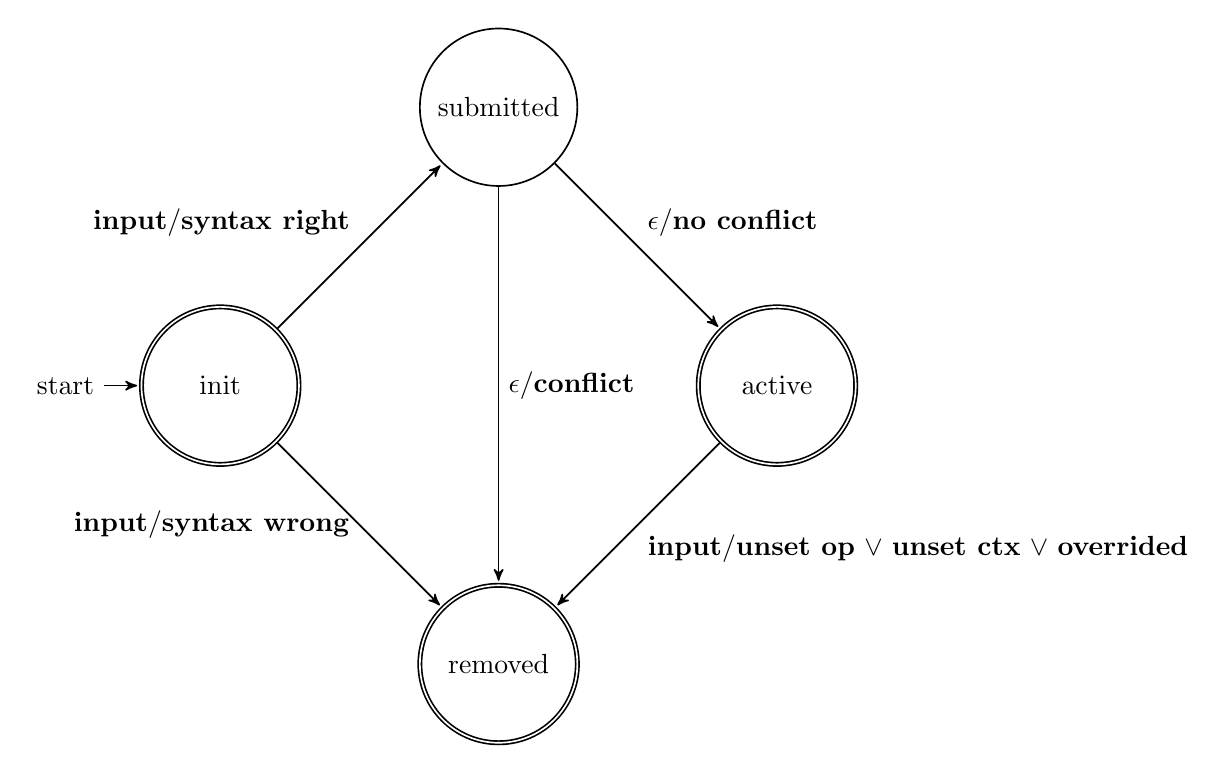
\begin{tikzpicture}[->,>=stealth',shorten >=1pt,auto,node distance=5cm,
                    semithick]
  \tikzstyle{every state}=[draw, text=black, circle, minimum size=2cm]

  \node[accepting, initial,state] (A)                    {init};
  \node[state]         (B) [above right of=A] {submitted};
  \node[accepting, state]         (C) [below right of=B] {active};
  \node[accepting, state]         (D) [below left of=C]  {removed};

  \path (A) edge              node {\textbf{input}/\textbf{syntax right}} (B)
        (A) edge[left]              node {\textbf{input}/\textbf{syntax wrong}} (D)
        (B) edge              node {\textbf{$\epsilon$}/\textbf{no conflict}} (C)
        (B) edge              node {\textbf{$\epsilon$}/\textbf{conflict}} (D)
        (C) edge           node {\textbf{input}/\textbf{unset op} $\lor$ \textbf{unset ctx} $\lor$ \textbf{overrided}} (D);
\end{tikzpicture}


当我们input一个指令的时候,该指令可能会改变之前指令的状态(使得之前指令的转移条件满足),该指令的状态转移依赖于之前的指令(转移条件中依赖之前指令的状态)。

\subsection{转移条件的具体定义}

TODO

\subsection{Reduction 自动机的性质}
从reduction自动机的转移函数中,我们可以推出以下3个非常重要的性质。

设新指令为 $\textbf{c}_{new}$, 之前指令为{$\textbf{c}_{old}$}, $\textbf{c}_{new}$ 转移依赖的之前指令为\{$\textbf{c}_{dep}$\}, $\textbf{c}_{new}$ 导致之前指令的指令状态发生改变 \{$\textbf{c}_{change}$\},这条指令加入后全部状态发生改变的指令 $\{\textbf{c}_{change}\}_{total}$

1. 新指令不会改变其状态转移依赖的指令, 即 $\{\textbf{c}_{dep}\} \cap  \{\textbf{c}_{change}\} = \emptyset$

2. 之前被改变的指令不会造成新的之前的指令被改变,即 $\{\textbf{c}_{change}\}_{total} = \{\textbf{c}_{change}\} \cup \textbf{c}_{new}$

3. 一条指令只会在它为最新指令时改变状态或者被当前最新指令改变状态,这两种情况每种最多造成一次状态改变。

\textbf{证明略,可以对根据自动机的结构对转移条件做归纳证明}

\subsection{Reduction 算法}
\begin{algorithm}
\caption{Reduction algorithm}
\begin{algorithmic}[1]
\Require OSPF configure $\textbf{conf}$
\Ensure Normal form of configure $\textbf{conf}_{norm}$
\State Initialize $\sigma \gets \{\textbf{c} \rightsquigarrow \textbf{INIT} | \textbf{c} \in \text{conf}\}$  \Comment{$\sigma$ stores state of each command}
\State Initialize $\textbf{conf}_{norm}$ to empty
\For{each command $c^l$ in \text{conf}}
    \State $\sigma \gets \text{move}(conf[:l-1], c^l, \sigma)$ \Comment{Update $\sigma$ with new states}
\EndFor
\For{each command $c^l$ in \text{conf}}
    \If{$\sigma[c^l]={\textbf{active}}$}
        \State add $c^l$ to $\textbf{conf}_{norm}$
    \EndIf
\EndFor
\end{algorithmic}
\end{algorithm}

% \begin{algorithm}
% \caption{move function}
% \begin{algorithmic}[1]
% \Require OSPF previous configure $\textbf{conf}$, current command $c^l$, states store $\sigma$
% \Ensure new states store $\sigma'$ after states update
% \end{algorithmic}
% \end{algorithm}

\end{document}